\documentclass{elsarticle}
\usepackage{graphicx, color}
\newcommand{\hlnumber}[1]{\textcolor[rgb]{0,0,0}{#1}}%
\newcommand{\hlfunctioncall}[1]{\textcolor[rgb]{.5,0,.33}{\textbf{#1}}}%
\newcommand{\hlstring}[1]{\textcolor[rgb]{.6,.6,1}{#1}}%
\newcommand{\hlkeyword}[1]{\textbf{#1}}%
\newcommand{\hlargument}[1]{\textcolor[rgb]{.69,.25,.02}{#1}}%
\newcommand{\hlcomment}[1]{\textcolor[rgb]{.18,.6,.34}{#1}}%
\newcommand{\hlroxygencomment}[1]{\textcolor[rgb]{.44,.48,.7}{#1}}%
\newcommand{\hlformalargs}[1]{\hlargument{#1}}%
\newcommand{\hleqformalargs}[1]{\hlargument{#1}}%
\newcommand{\hlassignement}[1]{\textbf{#1}}%
\newcommand{\hlpackage}[1]{\textcolor[rgb]{.59,.71,.145}{#1}}%
\newcommand{\hlslot}[1]{\textit{#1}}%
\newcommand{\hlsymbol}[1]{#1}%
\newcommand{\hlprompt}[1]{\textcolor[rgb]{.5,.5,.5}{#1}}%

\usepackage{color}%
 
\newsavebox{\hlnormalsizeboxclosebrace}%
\newsavebox{\hlnormalsizeboxopenbrace}%
\newsavebox{\hlnormalsizeboxbackslash}%
\newsavebox{\hlnormalsizeboxlessthan}%
\newsavebox{\hlnormalsizeboxgreaterthan}%
\newsavebox{\hlnormalsizeboxdollar}%
\newsavebox{\hlnormalsizeboxunderscore}%
\newsavebox{\hlnormalsizeboxand}%
\newsavebox{\hlnormalsizeboxhash}%
\newsavebox{\hlnormalsizeboxat}%
\newsavebox{\hlnormalsizeboxpercent}% 
\newsavebox{\hlnormalsizeboxhat}%
\newsavebox{\hlnormalsizeboxsinglequote}%
\newsavebox{\hlnormalsizeboxbacktick}%

\setbox\hlnormalsizeboxopenbrace=\hbox{\begin{normalsize}\verb.{.\end{normalsize}}%
\setbox\hlnormalsizeboxclosebrace=\hbox{\begin{normalsize}\verb.}.\end{normalsize}}%
\setbox\hlnormalsizeboxlessthan=\hbox{\begin{normalsize}\verb.<.\end{normalsize}}%
\setbox\hlnormalsizeboxdollar=\hbox{\begin{normalsize}\verb.$.\end{normalsize}}%
\setbox\hlnormalsizeboxunderscore=\hbox{\begin{normalsize}\verb._.\end{normalsize}}%
\setbox\hlnormalsizeboxand=\hbox{\begin{normalsize}\verb.&.\end{normalsize}}%
\setbox\hlnormalsizeboxhash=\hbox{\begin{normalsize}\verb.#.\end{normalsize}}%
\setbox\hlnormalsizeboxat=\hbox{\begin{normalsize}\verb.@.\end{normalsize}}%
\setbox\hlnormalsizeboxbackslash=\hbox{\begin{normalsize}\verb.\.\end{normalsize}}%
\setbox\hlnormalsizeboxgreaterthan=\hbox{\begin{normalsize}\verb.>.\end{normalsize}}%
\setbox\hlnormalsizeboxpercent=\hbox{\begin{normalsize}\verb.%.\end{normalsize}}%
\setbox\hlnormalsizeboxhat=\hbox{\begin{normalsize}\verb.^.\end{normalsize}}%
\setbox\hlnormalsizeboxsinglequote=\hbox{\begin{normalsize}\verb.'.\end{normalsize}}%
\setbox\hlnormalsizeboxbacktick=\hbox{\begin{normalsize}\verb.`.\end{normalsize}}%
\setbox\hlnormalsizeboxhat=\hbox{\begin{normalsize}\verb.^.\end{normalsize}}%



\newsavebox{\hltinyboxclosebrace}%
\newsavebox{\hltinyboxopenbrace}%
\newsavebox{\hltinyboxbackslash}%
\newsavebox{\hltinyboxlessthan}%
\newsavebox{\hltinyboxgreaterthan}%
\newsavebox{\hltinyboxdollar}%
\newsavebox{\hltinyboxunderscore}%
\newsavebox{\hltinyboxand}%
\newsavebox{\hltinyboxhash}%
\newsavebox{\hltinyboxat}%
\newsavebox{\hltinyboxpercent}% 
\newsavebox{\hltinyboxhat}%
\newsavebox{\hltinyboxsinglequote}%
\newsavebox{\hltinyboxbacktick}%

\setbox\hltinyboxopenbrace=\hbox{\begin{tiny}\verb.{.\end{tiny}}%
\setbox\hltinyboxclosebrace=\hbox{\begin{tiny}\verb.}.\end{tiny}}%
\setbox\hltinyboxlessthan=\hbox{\begin{tiny}\verb.<.\end{tiny}}%
\setbox\hltinyboxdollar=\hbox{\begin{tiny}\verb.$.\end{tiny}}%
\setbox\hltinyboxunderscore=\hbox{\begin{tiny}\verb._.\end{tiny}}%
\setbox\hltinyboxand=\hbox{\begin{tiny}\verb.&.\end{tiny}}%
\setbox\hltinyboxhash=\hbox{\begin{tiny}\verb.#.\end{tiny}}%
\setbox\hltinyboxat=\hbox{\begin{tiny}\verb.@.\end{tiny}}%
\setbox\hltinyboxbackslash=\hbox{\begin{tiny}\verb.\.\end{tiny}}%
\setbox\hltinyboxgreaterthan=\hbox{\begin{tiny}\verb.>.\end{tiny}}%
\setbox\hltinyboxpercent=\hbox{\begin{tiny}\verb.%.\end{tiny}}%
\setbox\hltinyboxhat=\hbox{\begin{tiny}\verb.^.\end{tiny}}%
\setbox\hltinyboxsinglequote=\hbox{\begin{tiny}\verb.'.\end{tiny}}%
\setbox\hltinyboxbacktick=\hbox{\begin{tiny}\verb.`.\end{tiny}}%
\setbox\hltinyboxhat=\hbox{\begin{tiny}\verb.^.\end{tiny}}%



\newsavebox{\hlscriptsizeboxclosebrace}%
\newsavebox{\hlscriptsizeboxopenbrace}%
\newsavebox{\hlscriptsizeboxbackslash}%
\newsavebox{\hlscriptsizeboxlessthan}%
\newsavebox{\hlscriptsizeboxgreaterthan}%
\newsavebox{\hlscriptsizeboxdollar}%
\newsavebox{\hlscriptsizeboxunderscore}%
\newsavebox{\hlscriptsizeboxand}%
\newsavebox{\hlscriptsizeboxhash}%
\newsavebox{\hlscriptsizeboxat}%
\newsavebox{\hlscriptsizeboxpercent}% 
\newsavebox{\hlscriptsizeboxhat}%
\newsavebox{\hlscriptsizeboxsinglequote}%
\newsavebox{\hlscriptsizeboxbacktick}%

\setbox\hlscriptsizeboxopenbrace=\hbox{\begin{scriptsize}\verb.{.\end{scriptsize}}%
\setbox\hlscriptsizeboxclosebrace=\hbox{\begin{scriptsize}\verb.}.\end{scriptsize}}%
\setbox\hlscriptsizeboxlessthan=\hbox{\begin{scriptsize}\verb.<.\end{scriptsize}}%
\setbox\hlscriptsizeboxdollar=\hbox{\begin{scriptsize}\verb.$.\end{scriptsize}}%
\setbox\hlscriptsizeboxunderscore=\hbox{\begin{scriptsize}\verb._.\end{scriptsize}}%
\setbox\hlscriptsizeboxand=\hbox{\begin{scriptsize}\verb.&.\end{scriptsize}}%
\setbox\hlscriptsizeboxhash=\hbox{\begin{scriptsize}\verb.#.\end{scriptsize}}%
\setbox\hlscriptsizeboxat=\hbox{\begin{scriptsize}\verb.@.\end{scriptsize}}%
\setbox\hlscriptsizeboxbackslash=\hbox{\begin{scriptsize}\verb.\.\end{scriptsize}}%
\setbox\hlscriptsizeboxgreaterthan=\hbox{\begin{scriptsize}\verb.>.\end{scriptsize}}%
\setbox\hlscriptsizeboxpercent=\hbox{\begin{scriptsize}\verb.%.\end{scriptsize}}%
\setbox\hlscriptsizeboxhat=\hbox{\begin{scriptsize}\verb.^.\end{scriptsize}}%
\setbox\hlscriptsizeboxsinglequote=\hbox{\begin{scriptsize}\verb.'.\end{scriptsize}}%
\setbox\hlscriptsizeboxbacktick=\hbox{\begin{scriptsize}\verb.`.\end{scriptsize}}%
\setbox\hlscriptsizeboxhat=\hbox{\begin{scriptsize}\verb.^.\end{scriptsize}}%



\newsavebox{\hlfootnotesizeboxclosebrace}%
\newsavebox{\hlfootnotesizeboxopenbrace}%
\newsavebox{\hlfootnotesizeboxbackslash}%
\newsavebox{\hlfootnotesizeboxlessthan}%
\newsavebox{\hlfootnotesizeboxgreaterthan}%
\newsavebox{\hlfootnotesizeboxdollar}%
\newsavebox{\hlfootnotesizeboxunderscore}%
\newsavebox{\hlfootnotesizeboxand}%
\newsavebox{\hlfootnotesizeboxhash}%
\newsavebox{\hlfootnotesizeboxat}%
\newsavebox{\hlfootnotesizeboxpercent}% 
\newsavebox{\hlfootnotesizeboxhat}%
\newsavebox{\hlfootnotesizeboxsinglequote}%
\newsavebox{\hlfootnotesizeboxbacktick}%

\setbox\hlfootnotesizeboxopenbrace=\hbox{\begin{footnotesize}\verb.{.\end{footnotesize}}%
\setbox\hlfootnotesizeboxclosebrace=\hbox{\begin{footnotesize}\verb.}.\end{footnotesize}}%
\setbox\hlfootnotesizeboxlessthan=\hbox{\begin{footnotesize}\verb.<.\end{footnotesize}}%
\setbox\hlfootnotesizeboxdollar=\hbox{\begin{footnotesize}\verb.$.\end{footnotesize}}%
\setbox\hlfootnotesizeboxunderscore=\hbox{\begin{footnotesize}\verb._.\end{footnotesize}}%
\setbox\hlfootnotesizeboxand=\hbox{\begin{footnotesize}\verb.&.\end{footnotesize}}%
\setbox\hlfootnotesizeboxhash=\hbox{\begin{footnotesize}\verb.#.\end{footnotesize}}%
\setbox\hlfootnotesizeboxat=\hbox{\begin{footnotesize}\verb.@.\end{footnotesize}}%
\setbox\hlfootnotesizeboxbackslash=\hbox{\begin{footnotesize}\verb.\.\end{footnotesize}}%
\setbox\hlfootnotesizeboxgreaterthan=\hbox{\begin{footnotesize}\verb.>.\end{footnotesize}}%
\setbox\hlfootnotesizeboxpercent=\hbox{\begin{footnotesize}\verb.%.\end{footnotesize}}%
\setbox\hlfootnotesizeboxhat=\hbox{\begin{footnotesize}\verb.^.\end{footnotesize}}%
\setbox\hlfootnotesizeboxsinglequote=\hbox{\begin{footnotesize}\verb.'.\end{footnotesize}}%
\setbox\hlfootnotesizeboxbacktick=\hbox{\begin{footnotesize}\verb.`.\end{footnotesize}}%
\setbox\hlfootnotesizeboxhat=\hbox{\begin{footnotesize}\verb.^.\end{footnotesize}}%



\newsavebox{\hlsmallboxclosebrace}%
\newsavebox{\hlsmallboxopenbrace}%
\newsavebox{\hlsmallboxbackslash}%
\newsavebox{\hlsmallboxlessthan}%
\newsavebox{\hlsmallboxgreaterthan}%
\newsavebox{\hlsmallboxdollar}%
\newsavebox{\hlsmallboxunderscore}%
\newsavebox{\hlsmallboxand}%
\newsavebox{\hlsmallboxhash}%
\newsavebox{\hlsmallboxat}%
\newsavebox{\hlsmallboxpercent}% 
\newsavebox{\hlsmallboxhat}%
\newsavebox{\hlsmallboxsinglequote}%
\newsavebox{\hlsmallboxbacktick}%

\setbox\hlsmallboxopenbrace=\hbox{\begin{small}\verb.{.\end{small}}%
\setbox\hlsmallboxclosebrace=\hbox{\begin{small}\verb.}.\end{small}}%
\setbox\hlsmallboxlessthan=\hbox{\begin{small}\verb.<.\end{small}}%
\setbox\hlsmallboxdollar=\hbox{\begin{small}\verb.$.\end{small}}%
\setbox\hlsmallboxunderscore=\hbox{\begin{small}\verb._.\end{small}}%
\setbox\hlsmallboxand=\hbox{\begin{small}\verb.&.\end{small}}%
\setbox\hlsmallboxhash=\hbox{\begin{small}\verb.#.\end{small}}%
\setbox\hlsmallboxat=\hbox{\begin{small}\verb.@.\end{small}}%
\setbox\hlsmallboxbackslash=\hbox{\begin{small}\verb.\.\end{small}}%
\setbox\hlsmallboxgreaterthan=\hbox{\begin{small}\verb.>.\end{small}}%
\setbox\hlsmallboxpercent=\hbox{\begin{small}\verb.%.\end{small}}%
\setbox\hlsmallboxhat=\hbox{\begin{small}\verb.^.\end{small}}%
\setbox\hlsmallboxsinglequote=\hbox{\begin{small}\verb.'.\end{small}}%
\setbox\hlsmallboxbacktick=\hbox{\begin{small}\verb.`.\end{small}}%
\setbox\hlsmallboxhat=\hbox{\begin{small}\verb.^.\end{small}}%



\newsavebox{\hllargeboxclosebrace}%
\newsavebox{\hllargeboxopenbrace}%
\newsavebox{\hllargeboxbackslash}%
\newsavebox{\hllargeboxlessthan}%
\newsavebox{\hllargeboxgreaterthan}%
\newsavebox{\hllargeboxdollar}%
\newsavebox{\hllargeboxunderscore}%
\newsavebox{\hllargeboxand}%
\newsavebox{\hllargeboxhash}%
\newsavebox{\hllargeboxat}%
\newsavebox{\hllargeboxpercent}% 
\newsavebox{\hllargeboxhat}%
\newsavebox{\hllargeboxsinglequote}%
\newsavebox{\hllargeboxbacktick}%

\setbox\hllargeboxopenbrace=\hbox{\begin{large}\verb.{.\end{large}}%
\setbox\hllargeboxclosebrace=\hbox{\begin{large}\verb.}.\end{large}}%
\setbox\hllargeboxlessthan=\hbox{\begin{large}\verb.<.\end{large}}%
\setbox\hllargeboxdollar=\hbox{\begin{large}\verb.$.\end{large}}%
\setbox\hllargeboxunderscore=\hbox{\begin{large}\verb._.\end{large}}%
\setbox\hllargeboxand=\hbox{\begin{large}\verb.&.\end{large}}%
\setbox\hllargeboxhash=\hbox{\begin{large}\verb.#.\end{large}}%
\setbox\hllargeboxat=\hbox{\begin{large}\verb.@.\end{large}}%
\setbox\hllargeboxbackslash=\hbox{\begin{large}\verb.\.\end{large}}%
\setbox\hllargeboxgreaterthan=\hbox{\begin{large}\verb.>.\end{large}}%
\setbox\hllargeboxpercent=\hbox{\begin{large}\verb.%.\end{large}}%
\setbox\hllargeboxhat=\hbox{\begin{large}\verb.^.\end{large}}%
\setbox\hllargeboxsinglequote=\hbox{\begin{large}\verb.'.\end{large}}%
\setbox\hllargeboxbacktick=\hbox{\begin{large}\verb.`.\end{large}}%
\setbox\hllargeboxhat=\hbox{\begin{large}\verb.^.\end{large}}%



\newsavebox{\hlLargeboxclosebrace}%
\newsavebox{\hlLargeboxopenbrace}%
\newsavebox{\hlLargeboxbackslash}%
\newsavebox{\hlLargeboxlessthan}%
\newsavebox{\hlLargeboxgreaterthan}%
\newsavebox{\hlLargeboxdollar}%
\newsavebox{\hlLargeboxunderscore}%
\newsavebox{\hlLargeboxand}%
\newsavebox{\hlLargeboxhash}%
\newsavebox{\hlLargeboxat}%
\newsavebox{\hlLargeboxpercent}% 
\newsavebox{\hlLargeboxhat}%
\newsavebox{\hlLargeboxsinglequote}%
\newsavebox{\hlLargeboxbacktick}%

\setbox\hlLargeboxopenbrace=\hbox{\begin{Large}\verb.{.\end{Large}}%
\setbox\hlLargeboxclosebrace=\hbox{\begin{Large}\verb.}.\end{Large}}%
\setbox\hlLargeboxlessthan=\hbox{\begin{Large}\verb.<.\end{Large}}%
\setbox\hlLargeboxdollar=\hbox{\begin{Large}\verb.$.\end{Large}}%
\setbox\hlLargeboxunderscore=\hbox{\begin{Large}\verb._.\end{Large}}%
\setbox\hlLargeboxand=\hbox{\begin{Large}\verb.&.\end{Large}}%
\setbox\hlLargeboxhash=\hbox{\begin{Large}\verb.#.\end{Large}}%
\setbox\hlLargeboxat=\hbox{\begin{Large}\verb.@.\end{Large}}%
\setbox\hlLargeboxbackslash=\hbox{\begin{Large}\verb.\.\end{Large}}%
\setbox\hlLargeboxgreaterthan=\hbox{\begin{Large}\verb.>.\end{Large}}%
\setbox\hlLargeboxpercent=\hbox{\begin{Large}\verb.%.\end{Large}}%
\setbox\hlLargeboxhat=\hbox{\begin{Large}\verb.^.\end{Large}}%
\setbox\hlLargeboxsinglequote=\hbox{\begin{Large}\verb.'.\end{Large}}%
\setbox\hlLargeboxbacktick=\hbox{\begin{Large}\verb.`.\end{Large}}%
\setbox\hlLargeboxhat=\hbox{\begin{Large}\verb.^.\end{Large}}%



\newsavebox{\hlLARGEboxclosebrace}%
\newsavebox{\hlLARGEboxopenbrace}%
\newsavebox{\hlLARGEboxbackslash}%
\newsavebox{\hlLARGEboxlessthan}%
\newsavebox{\hlLARGEboxgreaterthan}%
\newsavebox{\hlLARGEboxdollar}%
\newsavebox{\hlLARGEboxunderscore}%
\newsavebox{\hlLARGEboxand}%
\newsavebox{\hlLARGEboxhash}%
\newsavebox{\hlLARGEboxat}%
\newsavebox{\hlLARGEboxpercent}% 
\newsavebox{\hlLARGEboxhat}%
\newsavebox{\hlLARGEboxsinglequote}%
\newsavebox{\hlLARGEboxbacktick}%

\setbox\hlLARGEboxopenbrace=\hbox{\begin{LARGE}\verb.{.\end{LARGE}}%
\setbox\hlLARGEboxclosebrace=\hbox{\begin{LARGE}\verb.}.\end{LARGE}}%
\setbox\hlLARGEboxlessthan=\hbox{\begin{LARGE}\verb.<.\end{LARGE}}%
\setbox\hlLARGEboxdollar=\hbox{\begin{LARGE}\verb.$.\end{LARGE}}%
\setbox\hlLARGEboxunderscore=\hbox{\begin{LARGE}\verb._.\end{LARGE}}%
\setbox\hlLARGEboxand=\hbox{\begin{LARGE}\verb.&.\end{LARGE}}%
\setbox\hlLARGEboxhash=\hbox{\begin{LARGE}\verb.#.\end{LARGE}}%
\setbox\hlLARGEboxat=\hbox{\begin{LARGE}\verb.@.\end{LARGE}}%
\setbox\hlLARGEboxbackslash=\hbox{\begin{LARGE}\verb.\.\end{LARGE}}%
\setbox\hlLARGEboxgreaterthan=\hbox{\begin{LARGE}\verb.>.\end{LARGE}}%
\setbox\hlLARGEboxpercent=\hbox{\begin{LARGE}\verb.%.\end{LARGE}}%
\setbox\hlLARGEboxhat=\hbox{\begin{LARGE}\verb.^.\end{LARGE}}%
\setbox\hlLARGEboxsinglequote=\hbox{\begin{LARGE}\verb.'.\end{LARGE}}%
\setbox\hlLARGEboxbacktick=\hbox{\begin{LARGE}\verb.`.\end{LARGE}}%
\setbox\hlLARGEboxhat=\hbox{\begin{LARGE}\verb.^.\end{LARGE}}%



\newsavebox{\hlhugeboxclosebrace}%
\newsavebox{\hlhugeboxopenbrace}%
\newsavebox{\hlhugeboxbackslash}%
\newsavebox{\hlhugeboxlessthan}%
\newsavebox{\hlhugeboxgreaterthan}%
\newsavebox{\hlhugeboxdollar}%
\newsavebox{\hlhugeboxunderscore}%
\newsavebox{\hlhugeboxand}%
\newsavebox{\hlhugeboxhash}%
\newsavebox{\hlhugeboxat}%
\newsavebox{\hlhugeboxpercent}% 
\newsavebox{\hlhugeboxhat}%
\newsavebox{\hlhugeboxsinglequote}%
\newsavebox{\hlhugeboxbacktick}%

\setbox\hlhugeboxopenbrace=\hbox{\begin{huge}\verb.{.\end{huge}}%
\setbox\hlhugeboxclosebrace=\hbox{\begin{huge}\verb.}.\end{huge}}%
\setbox\hlhugeboxlessthan=\hbox{\begin{huge}\verb.<.\end{huge}}%
\setbox\hlhugeboxdollar=\hbox{\begin{huge}\verb.$.\end{huge}}%
\setbox\hlhugeboxunderscore=\hbox{\begin{huge}\verb._.\end{huge}}%
\setbox\hlhugeboxand=\hbox{\begin{huge}\verb.&.\end{huge}}%
\setbox\hlhugeboxhash=\hbox{\begin{huge}\verb.#.\end{huge}}%
\setbox\hlhugeboxat=\hbox{\begin{huge}\verb.@.\end{huge}}%
\setbox\hlhugeboxbackslash=\hbox{\begin{huge}\verb.\.\end{huge}}%
\setbox\hlhugeboxgreaterthan=\hbox{\begin{huge}\verb.>.\end{huge}}%
\setbox\hlhugeboxpercent=\hbox{\begin{huge}\verb.%.\end{huge}}%
\setbox\hlhugeboxhat=\hbox{\begin{huge}\verb.^.\end{huge}}%
\setbox\hlhugeboxsinglequote=\hbox{\begin{huge}\verb.'.\end{huge}}%
\setbox\hlhugeboxbacktick=\hbox{\begin{huge}\verb.`.\end{huge}}%
\setbox\hlhugeboxhat=\hbox{\begin{huge}\verb.^.\end{huge}}%



\newsavebox{\hlHugeboxclosebrace}%
\newsavebox{\hlHugeboxopenbrace}%
\newsavebox{\hlHugeboxbackslash}%
\newsavebox{\hlHugeboxlessthan}%
\newsavebox{\hlHugeboxgreaterthan}%
\newsavebox{\hlHugeboxdollar}%
\newsavebox{\hlHugeboxunderscore}%
\newsavebox{\hlHugeboxand}%
\newsavebox{\hlHugeboxhash}%
\newsavebox{\hlHugeboxat}%
\newsavebox{\hlHugeboxpercent}% 
\newsavebox{\hlHugeboxhat}%
\newsavebox{\hlHugeboxsinglequote}%
\newsavebox{\hlHugeboxbacktick}%

\setbox\hlHugeboxopenbrace=\hbox{\begin{Huge}\verb.{.\end{Huge}}%
\setbox\hlHugeboxclosebrace=\hbox{\begin{Huge}\verb.}.\end{Huge}}%
\setbox\hlHugeboxlessthan=\hbox{\begin{Huge}\verb.<.\end{Huge}}%
\setbox\hlHugeboxdollar=\hbox{\begin{Huge}\verb.$.\end{Huge}}%
\setbox\hlHugeboxunderscore=\hbox{\begin{Huge}\verb._.\end{Huge}}%
\setbox\hlHugeboxand=\hbox{\begin{Huge}\verb.&.\end{Huge}}%
\setbox\hlHugeboxhash=\hbox{\begin{Huge}\verb.#.\end{Huge}}%
\setbox\hlHugeboxat=\hbox{\begin{Huge}\verb.@.\end{Huge}}%
\setbox\hlHugeboxbackslash=\hbox{\begin{Huge}\verb.\.\end{Huge}}%
\setbox\hlHugeboxgreaterthan=\hbox{\begin{Huge}\verb.>.\end{Huge}}%
\setbox\hlHugeboxpercent=\hbox{\begin{Huge}\verb.%.\end{Huge}}%
\setbox\hlHugeboxhat=\hbox{\begin{Huge}\verb.^.\end{Huge}}%
\setbox\hlHugeboxsinglequote=\hbox{\begin{Huge}\verb.'.\end{Huge}}%
\setbox\hlHugeboxbacktick=\hbox{\begin{Huge}\verb.`.\end{Huge}}%
\setbox\hlHugeboxhat=\hbox{\begin{Huge}\verb.^.\end{Huge}}%
 

\def\urltilda{\kern -.15em\lower .7ex\hbox{\~{}}\kern .04em}%

\newcommand{\hlstd}[1]{\textcolor[rgb]{0,0,0}{#1}}%
\newcommand{\hlnum}[1]{\textcolor[rgb]{0.16,0.16,1}{#1}}
\newcommand{\hlesc}[1]{\textcolor[rgb]{1,0,1}{#1}}
\newcommand{\hlstr}[1]{\textcolor[rgb]{1,0,0}{#1}}
\newcommand{\hldstr}[1]{\textcolor[rgb]{0.51,0.51,0}{#1}}
\newcommand{\hlslc}[1]{\textcolor[rgb]{0.51,0.51,0.51}{\it{#1}}}
\newcommand{\hlcom}[1]{\textcolor[rgb]{0.51,0.51,0.51}{\it{#1}}}
\newcommand{\hldir}[1]{\textcolor[rgb]{0,0.51,0}{#1}}
\newcommand{\hlsym}[1]{\textcolor[rgb]{0,0,0}{#1}}
\newcommand{\hlline}[1]{\textcolor[rgb]{0.33,0.33,0.33}{#1}}
\newcommand{\hlkwa}[1]{\textcolor[rgb]{0,0,0}{\bf{#1}}}
\newcommand{\hlkwb}[1]{\textcolor[rgb]{0.51,0,0}{#1}}
\newcommand{\hlkwc}[1]{\textcolor[rgb]{0,0,0}{\bf{#1}}}
\newcommand{\hlkwd}[1]{\textcolor[rgb]{0,0,0.51}{#1}}

\definecolor{fgcolor}{rgb}{0,0,0}
\usepackage{framed}
\makeatletter
\newenvironment{kframe}{%
 \def\FrameCommand##1{\hskip\@totalleftmargin \hskip-\fboxsep
 \colorbox{shadecolor}{##1}\hskip-\fboxsep
     % There is no \@totalrightmargin, so:
     \hskip-\linewidth \hskip-\@totalleftmargin \hskip\columnwidth}%
 \MakeFramed {\advance\hsize-\width
   \@totalleftmargin\z@ \linewidth\hsize
   \@setminipage}}%
 {\par\unskip\endMakeFramed}
\makeatother

\newenvironment{knitrout}{}{} % an empty environment to be redefined in TeX


%\VignetteIndexEntry{treebase}
%% Redefines the elsarticle footer
\makeatletter
\def\ps@pprintTitle{%
 \let\@oddhead\@empty
 \let\@evenhead\@empty
 \def\@oddfoot{\it \hfill\today}%
 \let\@evenfoot\@oddfoot}
\makeatother

\bibliographystyle{elsarticle-harv}
\usepackage{graphicx}
\usepackage[pdftex, colorlinks]{hyperref}
\usepackage{amsmath, amsfonts}  % extended mathematics
\usepackage{booktabs} % book-quality tables

\textwidth 6.75in
\oddsidemargin -0.15in
\evensidemargin -0.15in
\textheight 9in
\topmargin -0.5in
\newcommand{\ud}{\mathrm{d}}


%% Looks like a comment but it isn't! This is setting the default behavior for the Sweave chunk options,  
% 

                   

\usepackage{Sweave}
\begin{document}
\begin{frontmatter}
  \title{An introduction to the \texttt{treebase} Package}
  \author[davis]{Carl Boettiger\corref{cor1}}
  \ead{cboettig@ucdavis.edu}
  \author[stats]{Duncan Temple Lang}
  \cortext[cor1]{Corresponding author.}
  \address[davis]{Center for Population Biology, University of California, Davis, United States}
  \address[stats]{Department of Statistics, University of California, Davis, United States}

  \begin{abstract}
  This paper describes the functionality provided by the software~\texttt{treebase},
  which provides an interface between the TreeBASE repository and the R programming language.  
  We illustrate how the package can be used to search and retrieve phylogenetic trees from the repository,
  replicate existing studies that have deposited their phylogenies on TreeBASE,
  and perform automatically-updatable meta-analyses across the repostory.  

  \end{abstract}

  \begin{keyword}
   R  \sep vignette \sep API \sep TreeBASE
   \end{keyword}
 \end{frontmatter}

\section{Introduction}
Applications that use phylogenetic information as part of their analyses 
are becoming increasingly central to both evolutionary and ecological research. 
The explosion of genomic data, followed by methodological advances for inferring phylogenies from this molecular information,
have helped spur this increase.
The R statistical environment has become the dominant platform for researchers performing applied phylogenetic methods
(27 are listed on the taskview on Phylogenetic Methods of the Comprehensive R Archive Network) 
and new methods are added every year.  

TreeBASE is an online repository of phylogenies~\citep{Sanderson1994b}.  
With the advent of mandatory data archiving in many of the major journals publishing phylognetics-based research 
over the past year~\citep{Fairbairn2010, Piwowar2011, Whitlock2010}, 
such resources can expect to become increasingly prominent.  
TreeBASE provides an application programming interface, or API, that lets applications make queries to the database.  
We have implemented an R package that plugs into this interface to provide direct access to this data.  

\section{Examples \& Results}





The basic functions of the TreeBASE API allow search queries of the phylogenetic data in the repository
(using the phylo-ws interface) and the metadata of publications associated with the phylogenies (using the OAI-MPH interface).
These interfaces are well-documented on the TreeBASE website.
The \texttt{treebase} package allows these queries to be made directly from R,
just as a user would make them from the browser.
The real advantage of the capacity to automate these tasks in R is shown in the later examples on replicating results and performing meta-analyses, but first, we introduce the package with some simple examples.  


\subsection{Basic Queries}
Any of the basic queries avaiable on the web interface can now be made directly from R,
including downloading and importing the phylogeny into the R interface.  
For instance, the following command searches for phylogenies containing dolphins,
or all phylogenies submitted by a given author
\begin{knitrout}
\definecolor{shadecolor}{rgb}{.97, .97, .97}{\color{fgcolor}\begin{kframe}
\begin{flushleft}
\ttfamily\noindent
\hlfunctioncall{search\usebox{\hlnormalsizeboxunderscore}treebase}\hlkeyword{(}\hlstring{"{}\usebox{\hlnormalsizeboxbackslash}"{}Delphinus\usebox{\hlnormalsizeboxbackslash}"{}"{}}\hlkeyword{,}{\ }\hlargument{by}\hlargument{=}\hlstring{"{}taxon"{}}\hlkeyword{)}\hspace*{\fill}\\
\hlstd{}\hlfunctioncall{search\usebox{\hlnormalsizeboxunderscore}treebase}\hlkeyword{(}\hlstring{"{}Huelsenbeck"{}}\hlkeyword{,}{\ }\hlargument{by}\hlargument{=}\hlstring{"{}author"{}}\hlkeyword{)}\mbox{}
\normalfont
\end{flushleft}
\end{kframe}}
\end{knitrout}

which loads the matching phylogenies into R, ready for analysis.  
The package and online documentation provide many examples of other possible queries.  
The package also provides access to the metadata of all publications containing trees deposited in TreeBASE.
This can help the user discover phylogenies of interest and also allows the user to perform statistical analyses
on the data deposition itself. 
While the metadata can be searched within a given date range,
it is most straight-forward to import the full meta-data records first, with the command 
\begin{knitrout}
\definecolor{shadecolor}{rgb}{.97, .97, .97}{\color{fgcolor}\begin{kframe}
\begin{flushleft}
\ttfamily\noindent
\hlsymbol{metadata}{\ }\hlassignement{\usebox{\hlnormalsizeboxlessthan}-}{\ }\hlfunctioncall{search\usebox{\hlnormalsizeboxunderscore}metadata}\hlkeyword{(}\hlstring{"{}"{}}\hlkeyword{,}{\ }\hlargument{by}\hlargument{=}\hlstring{"{}all"{}}\hlkeyword{)}\mbox{}
\normalfont
\end{flushleft}
\end{kframe}}
\end{knitrout}

%For convience, it is possible to load the copy of this data cached at the time the package was compiled.  



\setkeys{Gin}{width=0.75\textwidth}
\begin{figure}
\begin{center}
\begin{knitrout}
\definecolor{shadecolor}{rgb}{.97, .97, .97}{\color{fgcolor}\begin{kframe}
\begin{flushleft}
\ttfamily\noindent
\hlsymbol{dates}{\ }\hlassignement{\usebox{\hlnormalsizeboxlessthan}-}{\ }\hlfunctioncall{sapply}\hlkeyword{(}\hlsymbol{metadata}\hlkeyword{,}{\ }\hlkeyword{function}\hlkeyword{(}\hlformalargs{x}\hlkeyword{)}{\ }\hlfunctioncall{as.numeric}\hlkeyword{(}\hlsymbol{x}\hlkeyword{\usebox{\hlnormalsizeboxdollar}}\hlsymbol{date}\hlkeyword{)}\hlkeyword{)}\hspace*{\fill}\\
\hlstd{}\hlfunctioncall{hist}\hlkeyword{(}\hlsymbol{dates}\hlkeyword{,}{\ }\hlargument{main}\hlargument{=}\hlstring{"{}TreeBase{\ }growth"{}}\hlkeyword{,}{\ }\hlargument{xlab}\hlargument{=}\hlstring{"{}Year"{}}\hlkeyword{)}\mbox{}
\normalfont
\end{flushleft}
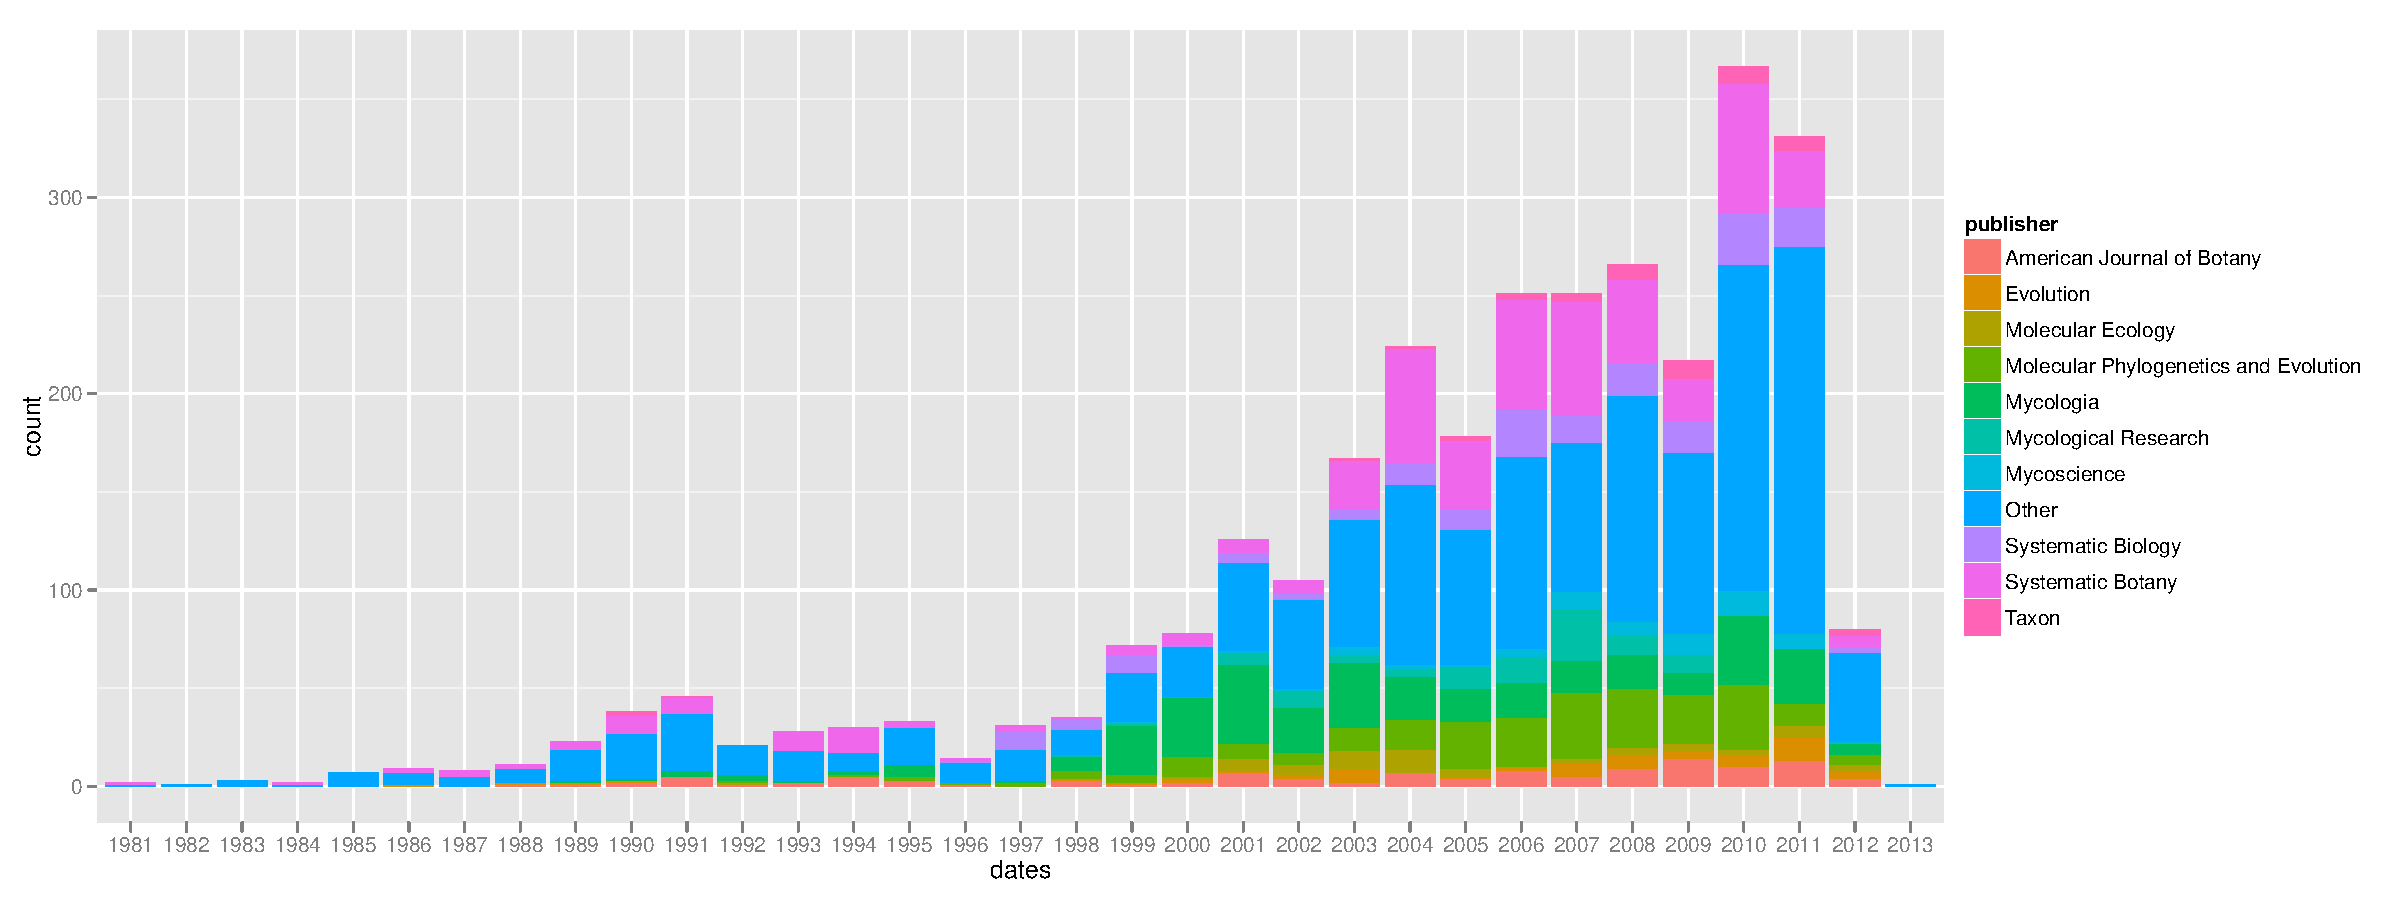
\includegraphics{dates} \end{kframe}}
\end{knitrout}

\caption{Histogram of publication dates by year, with the code required to generate the figure.}\label{fig:1}
\end{center}
\end{figure}
We can then look at the distribution of publication years for phylogenies depositied in TreeBASE and see if there is any trend, Fig~\ref{fig:1}. We can also look for patterns among publishers, such as comparing the number of submissions of two different publishers:
\begin{knitrout}
\definecolor{shadecolor}{rgb}{.97, .97, .97}{\color{fgcolor}\begin{kframe}
\begin{flushleft}
\ttfamily\noindent
\hlsymbol{nature}{\ }\hlassignement{\usebox{\hlnormalsizeboxlessthan}-}{\ }\hlfunctioncall{sapply}\hlkeyword{(}\hlsymbol{metadata}\hlkeyword{,}{\ }\hlkeyword{function}\hlkeyword{(}\hlformalargs{x}\hlkeyword{)}{\ }\hlfunctioncall{length}\hlkeyword{(}\hlfunctioncall{grep}\hlkeyword{(}\hlstring{"{}Nature"{}}\hlkeyword{,}{\ }\hlsymbol{x}\hlkeyword{\usebox{\hlnormalsizeboxdollar}}\hlsymbol{publisher}\hlkeyword{)}\hlkeyword{)}\hlkeyword{\usebox{\hlnormalsizeboxgreaterthan}}\hlnumber{0}\hlkeyword{)}\hspace*{\fill}\\
\hlstd{}\hlsymbol{science}{\ }\hlassignement{\usebox{\hlnormalsizeboxlessthan}-}{\ }\hlfunctioncall{sapply}\hlkeyword{(}\hlsymbol{metadata}\hlkeyword{,}{\ }\hlkeyword{function}\hlkeyword{(}\hlformalargs{x}\hlkeyword{)}{\ }\hlfunctioncall{length}\hlkeyword{(}\hlfunctioncall{grep}\hlkeyword{(}\hlstring{"{}\usebox{\hlnormalsizeboxhat}Science\usebox{\hlnormalsizeboxdollar}"{}}\hlkeyword{,}{\ }\hlsymbol{x}\hlkeyword{\usebox{\hlnormalsizeboxdollar}}\hlsymbol{publisher}\hlkeyword{)}\hlkeyword{)}\hlkeyword{\usebox{\hlnormalsizeboxgreaterthan}}\hlnumber{0}\hlkeyword{)}\mbox{}
\normalfont
\end{flushleft}
\end{kframe}}
\end{knitrout}

Summing the returned lists in each we find 15 phylogenies in \emph{Nature} and 14 in \emph{Science}. Many more such exercises are possible, and several examples are included in the demo files provided with the package.  

\subsection{Reproducible research \& education}
Reproducible research has become a topic of increasing concern in recent years~\citep{Schwab2000, Keiding2010a, Peng2011b}.  Access to data and executable scripts that reproduce the results presented are two central elements of this process which are addressed by the \texttt{treebase} package.   


\begin{knitrout}
\definecolor{shadecolor}{rgb}{.97, .97, .97}{\color{fgcolor}\begin{kframe}
\begin{flushleft}
\ttfamily\noindent
\hlsymbol{derryberry}{\ }\hlassignement{\usebox{\hlnormalsizeboxlessthan}-}{\ }\hlfunctioncall{search\usebox{\hlnormalsizeboxunderscore}treebase}\hlkeyword{(}\hlstring{"{}Derryberry"{}}\hlkeyword{,}{\ }\hlstring{"{}author"{}}\hlkeyword{)}\hlkeyword{[[}\hlnumber{1}\hlkeyword{]}\hlkeyword{]}\mbox{}
\normalfont
\end{flushleft}
\end{kframe}}
\end{knitrout}




% tree is too large to include a proper pretty plot.  metadata output is also too long to display nicely
\begin{knitrout}
\definecolor{shadecolor}{rgb}{.97, .97, .97}{\color{fgcolor}\begin{kframe}
\begin{flushleft}
\ttfamily\noindent
\hlfunctioncall{metadata}\hlkeyword{(}\hlsymbol{derryberry}\hlkeyword{\usebox{\hlnormalsizeboxdollar}}\hlsymbol{S.id}\hlkeyword{)}\hspace*{\fill}\\
\hlstd{}\hlfunctioncall{plot}\hlkeyword{(}\hlsymbol{derryberry}\hlkeyword{)}\mbox{}
\normalfont
\end{flushleft}
\end{kframe}}
\end{knitrout}


For instance, we can replicate the model choice methods they perform to select the most likely branching model candidate.  
\begin{knitrout}
\definecolor{shadecolor}{rgb}{.97, .97, .97}{\color{fgcolor}\begin{kframe}
\begin{flushleft}
\ttfamily\noindent
\hlfunctioncall{require}\hlkeyword{(}\hlsymbol{laser}\hlkeyword{)}\hspace*{\fill}\\
\hlstd{}\hlsymbol{tt}{\ }\hlassignement{\usebox{\hlnormalsizeboxlessthan}-}{\ }\hlfunctioncall{branching.times}\hlkeyword{(}\hlsymbol{derryberry}\hlkeyword{)}\hspace*{\fill}\\
\hlstd{}\hlsymbol{models}{\ }\hlassignement{\usebox{\hlnormalsizeboxlessthan}-}{\ }{\ }\hlfunctioncall{list}\hlkeyword{(}\hlargument{pb}{\ }\hlargument{=}{\ }\hlfunctioncall{pureBirth}\hlkeyword{(}\hlsymbol{tt}\hlkeyword{)}\hlkeyword{,}{\ }\hlcomment{\usebox{\hlnormalsizeboxhash}{\ }yule{\ }model}\hspace*{\fill}\\
\hlstd{}{\ }{\ }{\ }{\ }{\ }{\ }{\ }{\ }{\ }{\ }{\ }{\ }{\ }{\ }{\ }{\ }\hlargument{bdfit}{\ }\hlargument{=}{\ }\hlfunctioncall{bd}\hlkeyword{(}\hlsymbol{tt}\hlkeyword{)}\hlkeyword{,}{\ }\hlcomment{\usebox{\hlnormalsizeboxhash}{\ }birth-death{\ }model{\ }}\hspace*{\fill}\\
\hlstd{}{\ }{\ }{\ }{\ }{\ }{\ }{\ }{\ }{\ }{\ }{\ }{\ }{\ }{\ }{\ }{\ }\hlargument{y2r}{\ }\hlargument{=}{\ }\hlfunctioncall{yule2rate}\hlkeyword{(}\hlsymbol{tt}\hlkeyword{)}\hlkeyword{,}{\ }\hlcomment{\usebox{\hlnormalsizeboxhash}{\ }yule{\ }model{\ }with{\ }single{\ }shift{\ }pt}\hspace*{\fill}\\
\hlstd{}{\ }{\ }{\ }{\ }{\ }{\ }{\ }{\ }{\ }{\ }{\ }{\ }{\ }{\ }{\ }{\ }\hlargument{ddl}{\ }\hlargument{=}{\ }\hlfunctioncall{DDL}\hlkeyword{(}\hlsymbol{tt}\hlkeyword{)}\hlkeyword{,}{\ }\hlcomment{\usebox{\hlnormalsizeboxhash}{\ }linear,{\ }diversity-dependent}\hspace*{\fill}\\
\hlstd{}{\ }{\ }{\ }{\ }{\ }{\ }{\ }{\ }{\ }{\ }{\ }{\ }{\ }{\ }{\ }{\ }\hlargument{ddx}{\ }\hlargument{=}{\ }\hlfunctioncall{DDX}\hlkeyword{(}\hlsymbol{tt}\hlkeyword{)}\hlkeyword{,}{\ }\hlcomment{\usebox{\hlnormalsizeboxhash}exponential{\ }diversity-dendent}\hspace*{\fill}\\
\hlstd{}{\ }{\ }{\ }{\ }{\ }{\ }{\ }{\ }{\ }{\ }{\ }{\ }{\ }{\ }{\ }{\ }\hlargument{sv}{\ }\hlargument{=}{\ }\hlfunctioncall{fitSPVAR}\hlkeyword{(}\hlsymbol{tt}\hlkeyword{)}\hlkeyword{,}{\ }\hlcomment{\usebox{\hlnormalsizeboxhash}{\ }vary{\ }speciation{\ }in{\ }time}\hspace*{\fill}\\
\hlstd{}{\ }{\ }{\ }{\ }{\ }{\ }{\ }{\ }{\ }{\ }{\ }{\ }{\ }{\ }{\ }{\ }\hlargument{ev}{\ }\hlargument{=}{\ }\hlfunctioncall{fitEXVAR}\hlkeyword{(}\hlsymbol{tt}\hlkeyword{)}\hlkeyword{,}{\ }\hlcomment{\usebox{\hlnormalsizeboxhash}{\ }vary{\ }extinction{\ }in{\ }time}\hspace*{\fill}\\
\hlstd{}{\ }{\ }{\ }{\ }{\ }{\ }{\ }{\ }{\ }{\ }{\ }{\ }{\ }{\ }{\ }{\ }\hlargument{bv}{\ }\hlargument{=}{\ }\hlfunctioncall{fitBOTHVAR}\hlkeyword{(}\hlsymbol{tt}\hlkeyword{)}{\ }\hlcomment{\usebox{\hlnormalsizeboxhash}{\ }vary{\ }both}\hspace*{\fill}\\
\hlstd{}{\ }{\ }{\ }{\ }{\ }{\ }{\ }{\ }{\ }{\ }{\ }{\ }{\ }{\ }{\ }{\ }\hlkeyword{)}\hspace*{\fill}\\
\hlstd{}\hlsymbol{aics}{\ }\hlassignement{\usebox{\hlnormalsizeboxlessthan}-}{\ }\hlfunctioncall{sapply}\hlkeyword{(}\hlsymbol{models}\hlkeyword{,}{\ }\hlkeyword{function}\hlkeyword{(}\hlformalargs{x}\hlkeyword{)}{\ }\hlsymbol{x}\hlkeyword{\usebox{\hlnormalsizeboxdollar}}\hlsymbol{aic}\hlkeyword{)}\hspace*{\fill}\\
\hlstd{}\hlcomment{\usebox{\hlnormalsizeboxhash}{\ }name{\ }of{\ }the{\ }winning{\ }model}\hspace*{\fill}\\
\hlstd{}\hlfunctioncall{names}\hlkeyword{(}\hlsymbol{models}\hlkeyword{[}\hlfunctioncall{which.min}\hlkeyword{(}\hlsymbol{aics}\hlkeyword{)}\hlkeyword{]}\hlkeyword{)}\mbox{}
\normalfont
\end{flushleft}
\begin{verbatim}
## [1] "y2r"
\end{verbatim}
\end{kframe}}
\end{knitrout}


In this fast-moving field, new methods often become available within the timeframe that another manuscript is submitted by its authors and the time at which if first appears in print.  For instance, the more sophisticated methods avaialable in the more recent package, \texttt{TreePar}, were not used in this study. 





We can easily re-analyze these results using the TreePar software,
\begin{knitrout}
\definecolor{shadecolor}{rgb}{.97, .97, .97}{\color{fgcolor}\begin{kframe}
\begin{flushleft}
\ttfamily\noindent
{\ }{\ }{\ }{\ }{\ }\hlfunctioncall{require}\hlkeyword{(}\hlsymbol{TreePar}\hlkeyword{)}\hspace*{\fill}\\
\hlstd{}{\ }{\ }{\ }{\ }{\ }\hlsymbol{x}\hlassignement{\usebox{\hlnormalsizeboxlessthan}-}\hlfunctioncall{sort}\hlkeyword{(}\hlfunctioncall{getx}\hlkeyword{(}\hlsymbol{derryberry}\hlkeyword{)}\hlkeyword{,}\hlargument{decreasing}\hlargument{=}\hlnumber{TRUE}\hlkeyword{)}\hspace*{\fill}\\
\hlstd{}{\ }{\ }{\ }{\ }{\ }\hlcomment{\usebox{\hlnormalsizeboxhash}{\ }look{\ }for{\ }shifts{\ }occuring{\ }at{\ }times{\ }between{\ }0{\ }\usebox{\hlnormalsizeboxand}{\ }60{\ }with{\ }interval{\ }of{\ }5}\hspace*{\fill}\\
\hlstd{}{\ }{\ }{\ }{\ }{\ }\hlcomment{\usebox{\hlnormalsizeboxhash}{\ }consider{\ }yule{\ }models,{\ }allow{\ }up{\ }to{\ }3{\ }shifts{\ }(4{\ }different{\ }rates){\ }}\hspace*{\fill}\\
\hlstd{}{\ }{\ }{\ }{\ }{\ }\hlfunctioncall{invisible}\hlkeyword{(}\hlfunctioncall{capture.output}\hlkeyword{(}{\ }\hlcomment{\usebox{\hlnormalsizeboxhash}{\ }don\usebox{\hlnormalsizeboxsinglequote}t{\ }print{\ }messages}\hspace*{\fill}\\
\hlstd{}{\ }{\ }{\ }{\ }{\ }\hlsymbol{yule\usebox{\hlnormalsizeboxunderscore}4rate}{\ }\hlassignement{\usebox{\hlnormalsizeboxlessthan}-}{\ }\hlfunctioncall{bd.shifts.optim}\hlkeyword{(}\hlsymbol{x}\hlkeyword{,}\hlargument{sampling}\hlargument{=}\hlfunctioncall{c}\hlkeyword{(}\hlnumber{1}\hlkeyword{,}\hlnumber{1}\hlkeyword{,}\hlnumber{1}\hlkeyword{,}\hlnumber{1}\hlkeyword{)}\hlkeyword{,}\hspace*{\fill}\\
\hlstd{}{\ }{\ }{\ }{\ }{\ }{\ }{\ }{\ }{\ }{\ }{\ }{\ }{\ }{\ }{\ }{\ }{\ }{\ }{\ }{\ }{\ }{\ }{\ }{\ }{\ }{\ }{\ }{\ }{\ }{\ }{\ }{\ }{\ }{\ }{\ }\hlargument{grid}\hlargument{=}\hlnumber{5}\hlkeyword{,}\hlargument{start}\hlargument{=}\hlnumber{0}\hlkeyword{,}\hlargument{end}\hlargument{=}\hlnumber{60}\hlkeyword{,}\hlargument{ME}\hlargument{=}\hlnumber{FALSE}\hlkeyword{,}{\ }\hlargument{yule}\hlargument{=}\hlnumber{TRUE}\hlkeyword{)}\hlkeyword{)}\hlkeyword{)}\hspace*{\fill}\\
\hlstd{}{\ }{\ }{\ }{\ }{\ }\hlcomment{\usebox{\hlnormalsizeboxhash}{\ }yule\usebox{\hlnormalsizeboxunderscore}4rate[[2]][[i]]{\ }contains{\ }the{\ }-loglik{\ }and{\ }parameters{\ }}\hspace*{\fill}\\
\hlstd{}{\ }{\ }{\ }{\ }{\ }\hlcomment{\usebox{\hlnormalsizeboxhash}{\ }for{\ }"{}best{\ }soln{\ }on{\ }grid"{}{\ }for{\ }the{\ }model{\ }with{\ }i{\ }shifts}\hspace*{\fill}\\
\hlstd{}{\ }{\ }{\ }{\ }{\ }\hlsymbol{aic}{\ }\hlassignement{\usebox{\hlnormalsizeboxlessthan}-}{\ }\hlfunctioncall{sapply}\hlkeyword{(}\hlsymbol{yule\usebox{\hlnormalsizeboxunderscore}4rate}\hlkeyword{[[}\hlnumber{2}\hlkeyword{]}\hlkeyword{]}\hlkeyword{,}{\ }\hlkeyword{function}\hlkeyword{(}\hlformalargs{x}\hlkeyword{)}{\ }\hlnumber{2}{\ }\hlkeyword{*}{\ }\hlkeyword{(}\hlfunctioncall{length}\hlkeyword{(}\hlsymbol{x}\hlkeyword{)}{\ }\hlkeyword{-}{\ }\hlnumber{1}\hlkeyword{)}{\ }\hlkeyword{+}{\ }\hlnumber{2}{\ }\hlkeyword{*}{\ }\hlsymbol{x}\hlkeyword{[}\hlnumber{1}\hlkeyword{]}{\ }\hlkeyword{)}\hspace*{\fill}\\
\hlstd{}{\ }{\ }{\ }{\ }{\ }\hlfunctioncall{which.min}\hlkeyword{(}\hlsymbol{aic}\hlkeyword{)}\mbox{}
\normalfont
\end{flushleft}
\begin{verbatim}
##   
## 2 
\end{verbatim}
\end{kframe}}
\end{knitrout}

and confirm that the Yule 2-rate 
model is the best fitting by AIC score, 
even when allowing for up to four different shifts.  

\subsection{The self-updating meta-analysis}
Meta-analyses are becoming increasingly common in phylogenetic methods~\citep[\emph{e.g}][]{McPeek2007, Phillimore2008, McPeek2008,Quental2010, Davies2011a}.  
Accessing many phylogenies can be difficult, 
and researchers have gone through heroic efforts to extract phylogenetic information from the literature, 
such as~\citet{McPeek2007}, who report that 
``All branch lengths were measured by hand from these printed sheets using dial calipers'' 
on 163 phylogenies printed out from pdfs in which they appeared in the literature.  
Researchers may focus their meta-analysis on particular taxa~\citep{Phillimore2008}, 
leaving us to wonder if the conclusions hold in other groups.  
Other studies may use a single empirical tree accompanied by a a collection of simulated phylogenies~\citet{Cusimano2010}.  
Some already turn to TreeBASE to provide a more extensive collection of phylogenies~\citep{Davies2011a}.  
The analysis in many of these studies already uses or can use methods available in R.  

By building such meta-analyses around the \texttt{treebase} package, 
one can not only take advantage of the existing data with substantially less effort, 
but also provide a script that can be automatically updated as more phylogenies are deposited in the TreeBASE repository.  

\begin{knitrout}
\definecolor{shadecolor}{rgb}{.97, .97, .97}{\color{fgcolor}\begin{kframe}
\begin{flushleft}
\ttfamily\noindent
\hlsymbol{all\usebox{\hlnormalsizeboxunderscore}trees}{\ }\hlassignement{\usebox{\hlnormalsizeboxlessthan}-}{\ }\hlfunctioncall{search\usebox{\hlnormalsizeboxunderscore}treebase}\hlkeyword{(}\hlstring{"{}Consensus"{}}\hlkeyword{,}{\ }\hlstring{"{}type.tree"{}}\hlkeyword{,}{\ }\hlargument{branch\usebox{\hlnormalsizeboxunderscore}lengths}\hlargument{=}\hlnumber{TRUE}\hlkeyword{)}\mbox{}
\normalfont
\end{flushleft}
\end{kframe}}
\end{knitrout}


For convience and testing purposes, we could just load the cached set of all phylogenetic trees with branchlengths in TreeBASE at the time the package was built:
\begin{knitrout}
\definecolor{shadecolor}{rgb}{.97, .97, .97}{\color{fgcolor}\begin{kframe}
\begin{flushleft}
\ttfamily\noindent
\hlfunctioncall{data}\hlkeyword{(}\hlsymbol{branchlengths}\hlkeyword{)}\mbox{}
\normalfont
\end{flushleft}
\end{kframe}}
\end{knitrout}



Many meta-analyses require ultrametric trees (branch lengths proportional to time, rather than to mutational steps). 
This function is just an elementary example to illustrate the process of time-calibrating a tree;
more sophisticated methods could be chosen instead.  
\begin{knitrout}
\definecolor{shadecolor}{rgb}{.97, .97, .97}{\color{fgcolor}\begin{kframe}
\begin{flushleft}
\ttfamily\noindent
\hlsymbol{timetree}{\ }\hlassignement{\usebox{\hlnormalsizeboxlessthan}-}{\ }\hlkeyword{function}\hlkeyword{(}\hlformalargs{tree}\hlkeyword{)}\hlkeyword{\usebox{\hlnormalsizeboxopenbrace}}\hspace*{\fill}\\
\hlstd{}{\ }{\ }{\ }{\ }\hlsymbol{check.na}{\ }\hlassignement{\usebox{\hlnormalsizeboxlessthan}-}{\ }\hlfunctioncall{try}\hlkeyword{(}\hlfunctioncall{sum}\hlkeyword{(}\hlfunctioncall{is.na}\hlkeyword{(}\hlsymbol{tree}\hlkeyword{\usebox{\hlnormalsizeboxdollar}}\hlsymbol{edge.length}\hlkeyword{)}\hlkeyword{)}\hlkeyword{\usebox{\hlnormalsizeboxgreaterthan}}\hlnumber{0}\hlkeyword{)}\hspace*{\fill}\\
\hlstd{}{\ }{\ }{\ }{\ }\hlkeyword{if}\hlkeyword{(}\hlfunctioncall{is}\hlkeyword{(}\hlsymbol{check.na}\hlkeyword{,}{\ }\hlstring{"{}try-error"{}}\hlkeyword{)}{\ }\hlkeyword{|}{\ }\hlsymbol{check.na}\hlkeyword{)}\hspace*{\fill}\\
\hlstd{}{\ }{\ }{\ }{\ }{\ }{\ }NULL\hspace*{\fill}\\
\hlstd{}{\ }{\ }{\ }{\ }\hlkeyword{else}\hspace*{\fill}\\
\hlstd{}{\ }{\ }{\ }{\ }\hlfunctioncall{try}\hlkeyword{(}{\ }\hlfunctioncall{chronoMPL}\hlkeyword{(}\hlfunctioncall{multi2di}\hlkeyword{(}\hlsymbol{tree}\hlkeyword{)}\hlkeyword{)}{\ }\hlkeyword{)}\hspace*{\fill}\\
\hlstd{}\hlkeyword{\usebox{\hlnormalsizeboxclosebrace}}\hspace*{\fill}\\
\hlstd{}\hlsymbol{tt}{\ }\hlassignement{\usebox{\hlnormalsizeboxlessthan}-}{\ }\hlfunctioncall{drop\usebox{\hlnormalsizeboxunderscore}errors}\hlkeyword{(}\hlfunctioncall{sapply}\hlkeyword{(}\hlsymbol{branchlengths}\hlkeyword{,}{\ }\hlsymbol{timetree}\hlkeyword{)}\hlkeyword{)}\mbox{}
\normalfont
\end{flushleft}
\begin{verbatim}
## [1] "dropped 11 trees"
\end{verbatim}
\end{kframe}}
\end{knitrout}



The central question of many of meta-analyses mentioned above has been whether or not phylogenies show a changing rates of evolution.  A standard test of this is the $\gamma$ statistic of~\citet{Pybus2000} which tests the null hypothesis that the rates of speciation and extinction are constant.  Applying this test to all of the currently available trees in TreeBASE,
\begin{knitrout}
\definecolor{shadecolor}{rgb}{.97, .97, .97}{\color{fgcolor}\begin{kframe}
\begin{flushleft}
\ttfamily\noindent
\hlcomment{\usebox{\hlnormalsizeboxhash}{\ }gamma{\ }statistic}\hspace*{\fill}\\
\hlstd{}\hlsymbol{gammas}{\ }\hlassignement{\usebox{\hlnormalsizeboxlessthan}-}{\ }\hlfunctioncall{sapply}\hlkeyword{(}\hlsymbol{tt}\hlkeyword{,}{\ }\hlkeyword{function}\hlkeyword{(}\hlformalargs{phy}\hlkeyword{)}{\ }{\ }\hlfunctioncall{gammaStat}\hlkeyword{(}\hlsymbol{phy}\hlkeyword{)}\hlkeyword{)}\hspace*{\fill}\\
\hlstd{}\hlcomment{\usebox{\hlnormalsizeboxhash}{\ }associated{\ }p-value}\hspace*{\fill}\\
\hlstd{}\hlsymbol{p\usebox{\hlnormalsizeboxunderscore}gammas}{\ }\hlassignement{\usebox{\hlnormalsizeboxlessthan}-}{\ }\hlfunctioncall{sapply}\hlkeyword{(}\hlsymbol{gammas}\hlkeyword{,}{\ }\hlkeyword{function}\hlkeyword{(}\hlformalargs{x}\hlkeyword{)}{\ }{\ }\hlnumber{2}\hlkeyword{*}\hlkeyword{(}\hlnumber{1}\hlkeyword{-}\hlfunctioncall{pnorm}\hlkeyword{(}\hlfunctioncall{abs}\hlkeyword{(}\hlsymbol{x}\hlkeyword{)}\hlkeyword{)}\hlkeyword{)}\hlkeyword{)}\hspace*{\fill}\\
\hlstd{}\hlsymbol{non\usebox{\hlnormalsizeboxunderscore}const}{\ }\hlassignement{\usebox{\hlnormalsizeboxlessthan}-}{\ }\hlfunctioncall{sum}\hlkeyword{(}\hlsymbol{p\usebox{\hlnormalsizeboxunderscore}gammas}{\ }\hlkeyword{\usebox{\hlnormalsizeboxlessthan}}{\ }\hlnumber{0.025}\hlkeyword{)}\hlkeyword{/}\hlfunctioncall{length}\hlkeyword{(}\hlsymbol{gammas}\hlkeyword{)}\mbox{}
\normalfont
\end{flushleft}
\end{kframe}}
\end{knitrout}

we find that 54\% of the trees can reject the constant-rates model at the 95\% confidence level. 
Because \texttt{treebase} makes it possible to perform this analysis entirely by scripts using the latest treebase data, 
it is not only easier to perform this analysis but also to update it to reflect the latest data. 
For instance, this paper is written using R's Sweave tool, where the results and figures are generated on the fly as the paper is compiled.  
Consequently the analyses presented here can be updated to reflect the latest information in TreeBASE by the click of a button.  



 \section{Acknowledgements}
 CB wishes to thank the TreeBASE developer team for building and supporting the repository, and all contributers to TreeBASE.
 CB is supported by a Computational Sciences Graduate Fellowship from the Department of Energy under grant number DE-FG02-97ER25308.   
 \section*{ }%bibliography
% \bibliography{/home/cboettig/Documents/Mendeley/bib/library}
  \bibliography{treebase}

\end{document}


